\documentclass[11pt]{article}
\usepackage[textwidth=18.0cm, textheight=23.0cm, top=2.0cm]{geometry}
\usepackage{pst-all}
\usepackage{amssymb}
\usepackage{tikz}
\usepackage{underscore}\begin{document}
\pagestyle{empty}


ClassName: \underline{\textbf{Class_10.2bp-36}}
\par
BinSize: \underline{\textbf{100 × 100}}
\par
ReduceSize: \underline{\textbf{100 × 100}}
\par
TypeNum: \underline{\textbf{80}}
\par
Num: \underline{\textbf{80}}
\par
OutS: \underline{\textbf{140000}}
\par
InS: \underline{\textbf{133537}}
\par
Rate: \underline{\textbf{0.954}}
\par
UB: \underline{\textbf{14}}
\par
LB0: \underline{\textbf{14}}
\par
LB: \underline{\textbf{14}}
\par
LBWithCut: \underline{\textbf{14}}
\par
NodeCut: \underline{\textbf{0}}
\par
ExtendedNodeCnt: \underline{\textbf{1}}
\par
GenNodeCnt: \underline{\textbf{1}}
\par
PrimalNode: \underline{\textbf{0}}
\par
ColumnCount: \underline{\textbf{14}}
\par
TotalCutCount: \underline{\textbf{0}}
\par
RootCutCount: \underline{\textbf{0}}
\par
LPSolverCnt: \underline{\textbf{1}}
\par
PricingSolverCnt: \underline{\textbf{0}}
\par
BranchAndBoundNum: \underline{\textbf{1}}
\par
isOpt: \underline{\textbf{true}}
\par
TimeOnInitSolution: \underline{\textbf{600.000 s}}
\par
TimeOnPrimal: \underline{\textbf{0.000 s}}
\par
TimeOnPricing: \underline{\textbf{0.000 s}}
\par
TimeOnRmp: \underline{\textbf{0.063 s}}
\par
TotalTime: \underline{\textbf{600.328 s}}
\par
\newpage


\begin{tikzpicture}[shorten >=1pt,scale=1.0,every node/.style={scale=1.0},->]
\tikzstyle{vertex}=[circle,fill=black!25,minimum size=14pt,inner sep=0pt]
\filldraw[fill=gray!40!white, draw=black] (0,0) rectangle (15.0,15.0);
\foreach \name/\x/\y/\w/\h in {73x93/4.05/0.0/10.95/13.95,72x7/4.2/13.95/10.799999999999999/1.05,27x46/0.0/0.0/4.05/6.8999999999999995,26x38/0.15/6.8999999999999995/3.9/5.7,25x14/0.3/12.6/3.75/2.1,23x2/0.6/14.7/3.4499999999999997/0.3}
\filldraw[fill=white!40!white, draw=black] (\x,\y) rectangle node[draw] (\name) {\name} ++(\w,\h);
\end{tikzpicture}


w =73 , h =93 , x =27 , y =0 , v =6789
\par
w =72 , h =7 , x =28 , y =93 , v =504
\par
w =27 , h =46 , x =0 , y =0 , v =1242
\par
w =26 , h =38 , x =1 , y =46 , v =988
\par
w =25 , h =14 , x =2 , y =84 , v =350
\par
w =23 , h =2 , x =4 , y =98 , v =46
\par
\newpage


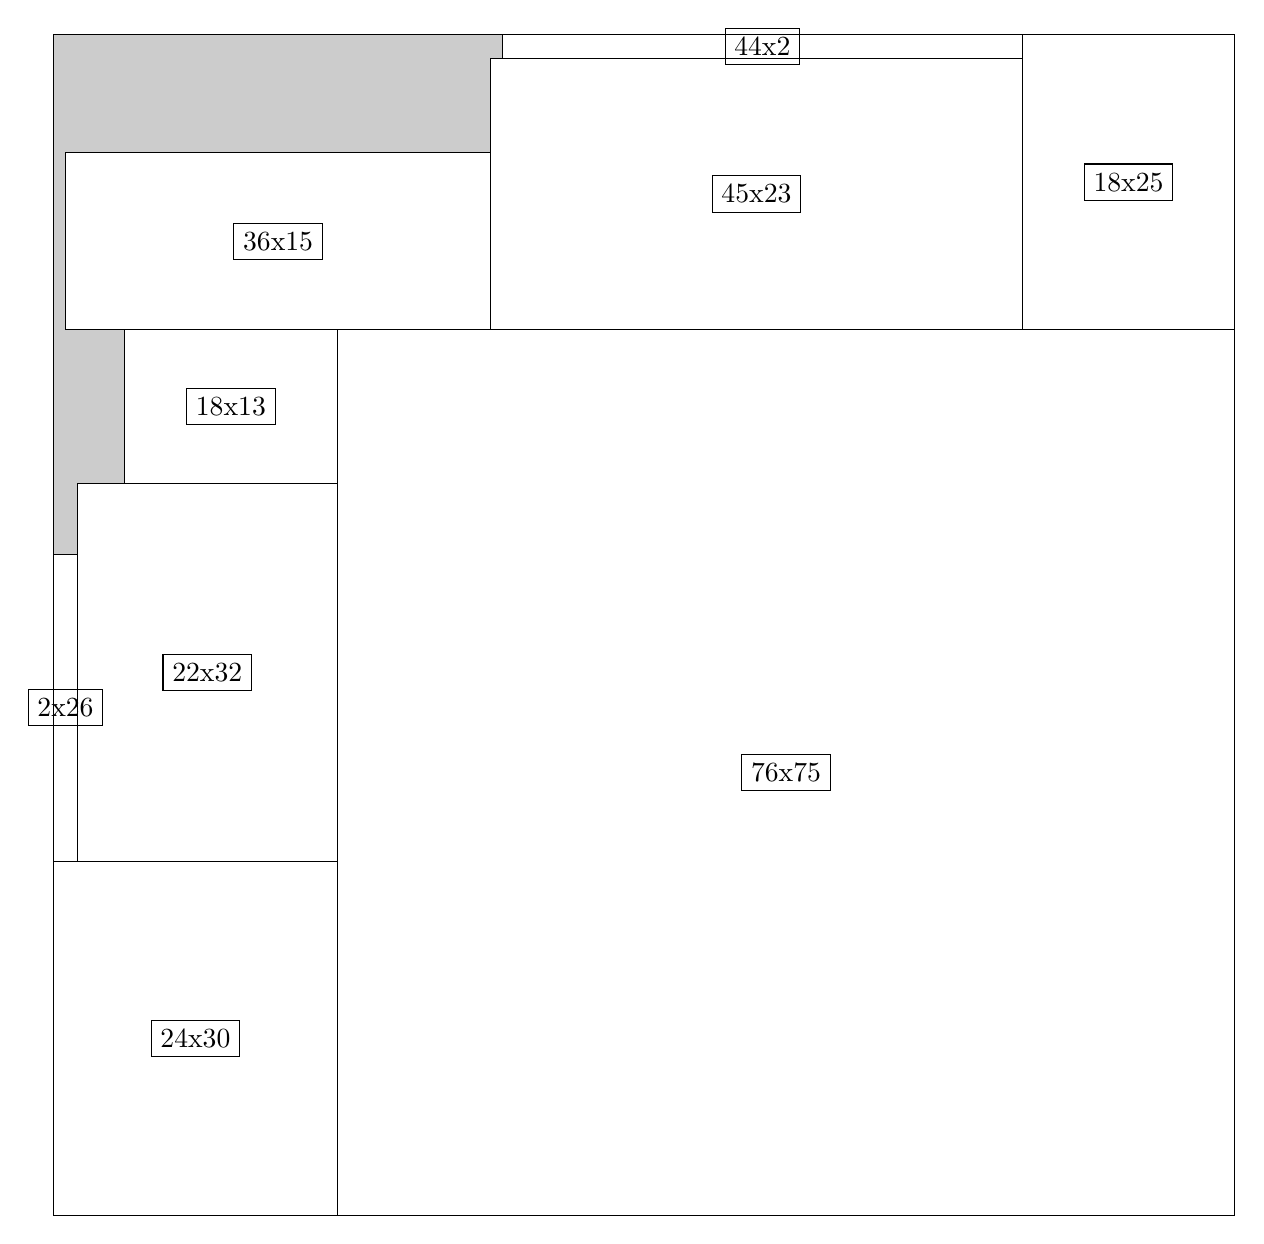
\begin{tikzpicture}[shorten >=1pt,scale=1.0,every node/.style={scale=1.0},->]
\tikzstyle{vertex}=[circle,fill=black!25,minimum size=14pt,inner sep=0pt]
\filldraw[fill=gray!40!white, draw=black] (0,0) rectangle (15.0,15.0);
\foreach \name/\x/\y/\w/\h in {76x75/3.5999999999999996/0.0/11.4/11.25,24x30/0.0/0.0/3.5999999999999996/4.5,22x32/0.3/4.5/3.3/4.8,2x26/0.0/4.5/0.3/3.9,18x13/0.8999999999999999/9.299999999999999/2.6999999999999997/1.95,18x25/12.299999999999999/11.25/2.6999999999999997/3.75,45x23/5.55/11.25/6.75/3.4499999999999997,44x2/5.7/14.7/6.6/0.3,36x15/0.15/11.25/5.3999999999999995/2.25}
\filldraw[fill=white!40!white, draw=black] (\x,\y) rectangle node[draw] (\name) {\name} ++(\w,\h);
\end{tikzpicture}


w =76 , h =75 , x =24 , y =0 , v =5700
\par
w =24 , h =30 , x =0 , y =0 , v =720
\par
w =22 , h =32 , x =2 , y =30 , v =704
\par
w =2 , h =26 , x =0 , y =30 , v =52
\par
w =18 , h =13 , x =6 , y =62 , v =234
\par
w =18 , h =25 , x =82 , y =75 , v =450
\par
w =45 , h =23 , x =37 , y =75 , v =1035
\par
w =44 , h =2 , x =38 , y =98 , v =88
\par
w =36 , h =15 , x =1 , y =75 , v =540
\par
\newpage


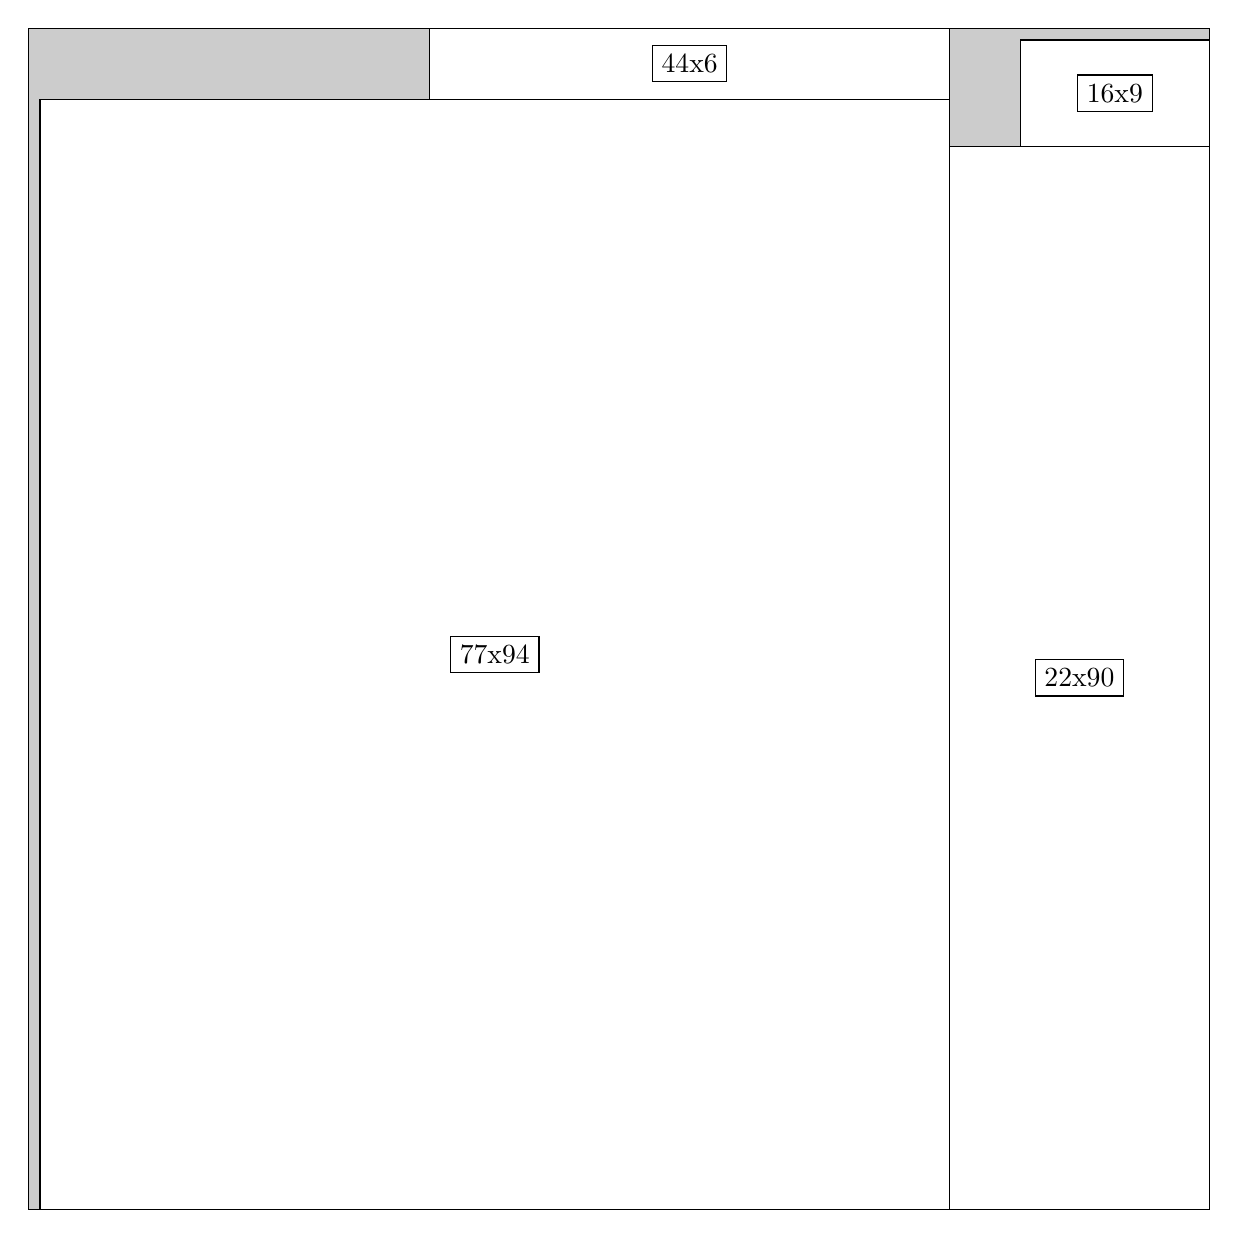
\begin{tikzpicture}[shorten >=1pt,scale=1.0,every node/.style={scale=1.0},->]
\tikzstyle{vertex}=[circle,fill=black!25,minimum size=14pt,inner sep=0pt]
\filldraw[fill=gray!40!white, draw=black] (0,0) rectangle (15.0,15.0);
\foreach \name/\x/\y/\w/\h in {22x90/11.7/0.0/3.3/13.5,16x9/12.6/13.5/2.4/1.3499999999999999,77x94/0.15/0.0/11.549999999999999/14.1,44x6/5.1/14.1/6.6/0.8999999999999999}
\filldraw[fill=white!40!white, draw=black] (\x,\y) rectangle node[draw] (\name) {\name} ++(\w,\h);
\end{tikzpicture}


w =22 , h =90 , x =78 , y =0 , v =1980
\par
w =16 , h =9 , x =84 , y =90 , v =144
\par
w =77 , h =94 , x =1 , y =0 , v =7238
\par
w =44 , h =6 , x =34 , y =94 , v =264
\par
\newpage


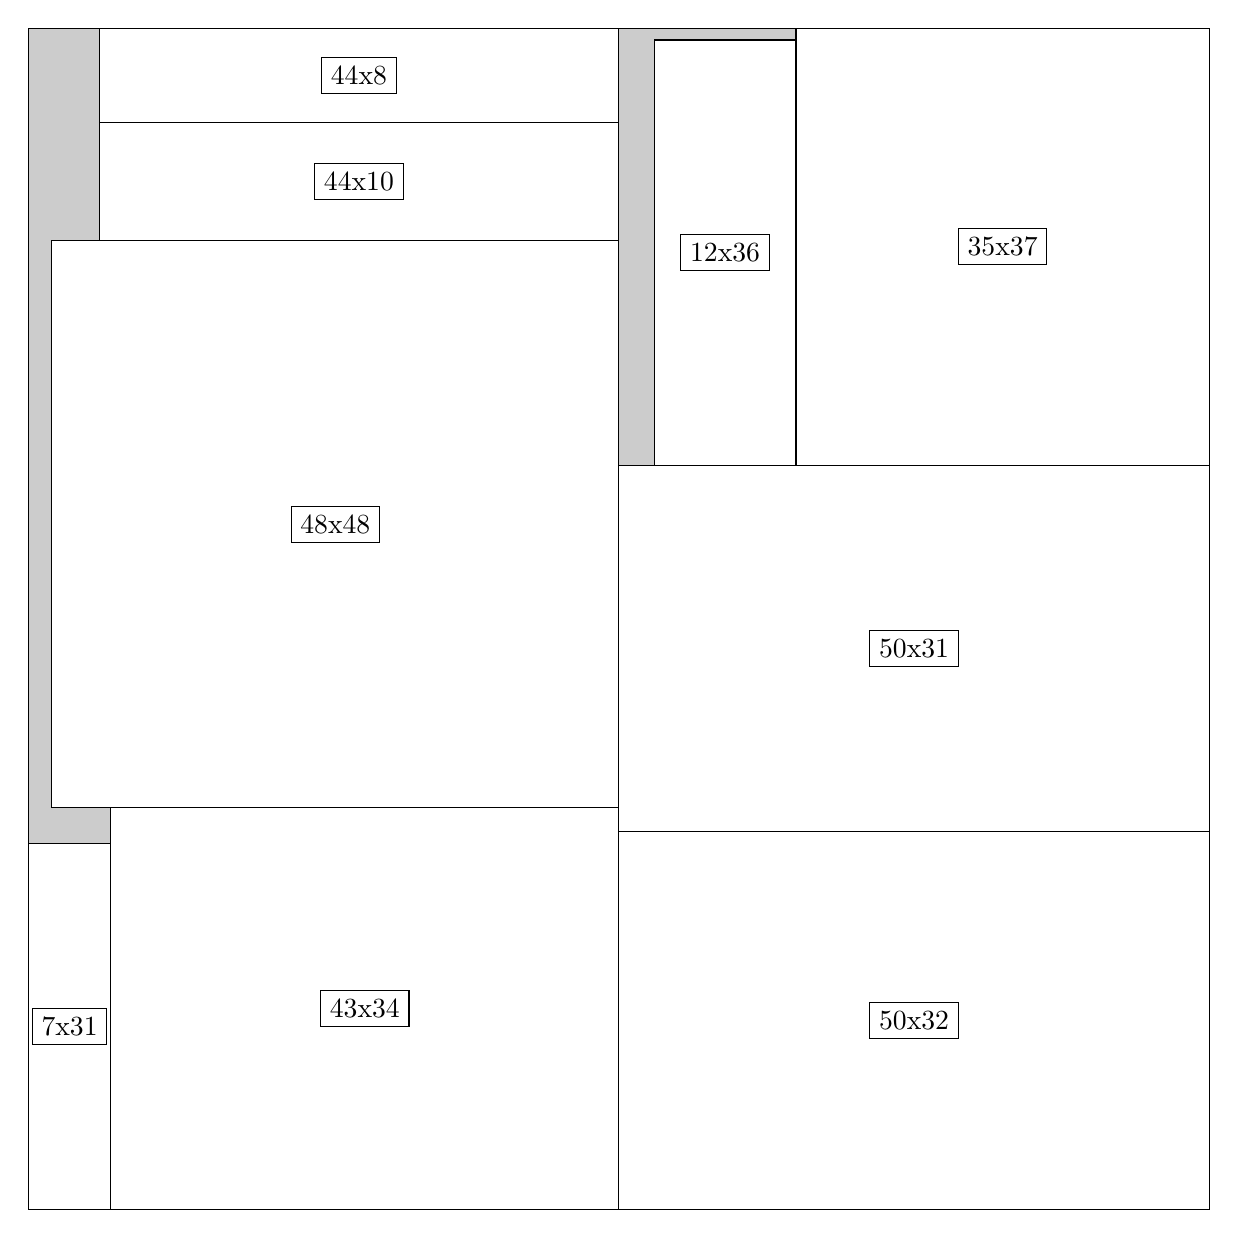
\begin{tikzpicture}[shorten >=1pt,scale=1.0,every node/.style={scale=1.0},->]
\tikzstyle{vertex}=[circle,fill=black!25,minimum size=14pt,inner sep=0pt]
\filldraw[fill=gray!40!white, draw=black] (0,0) rectangle (15.0,15.0);
\foreach \name/\x/\y/\w/\h in {50x32/7.5/0.0/7.5/4.8,50x31/7.5/4.8/7.5/4.6499999999999995,35x37/9.75/9.45/5.25/5.55,12x36/7.949999999999999/9.45/1.7999999999999998/5.3999999999999995,43x34/1.05/0.0/6.45/5.1,7x31/0.0/0.0/1.05/4.6499999999999995,48x48/0.3/5.1/7.199999999999999/7.199999999999999,44x10/0.8999999999999999/12.299999999999999/6.6/1.5,44x8/0.8999999999999999/13.799999999999999/6.6/1.2}
\filldraw[fill=white!40!white, draw=black] (\x,\y) rectangle node[draw] (\name) {\name} ++(\w,\h);
\end{tikzpicture}


w =50 , h =32 , x =50 , y =0 , v =1600
\par
w =50 , h =31 , x =50 , y =32 , v =1550
\par
w =35 , h =37 , x =65 , y =63 , v =1295
\par
w =12 , h =36 , x =53 , y =63 , v =432
\par
w =43 , h =34 , x =7 , y =0 , v =1462
\par
w =7 , h =31 , x =0 , y =0 , v =217
\par
w =48 , h =48 , x =2 , y =34 , v =2304
\par
w =44 , h =10 , x =6 , y =82 , v =440
\par
w =44 , h =8 , x =6 , y =92 , v =352
\par
\newpage


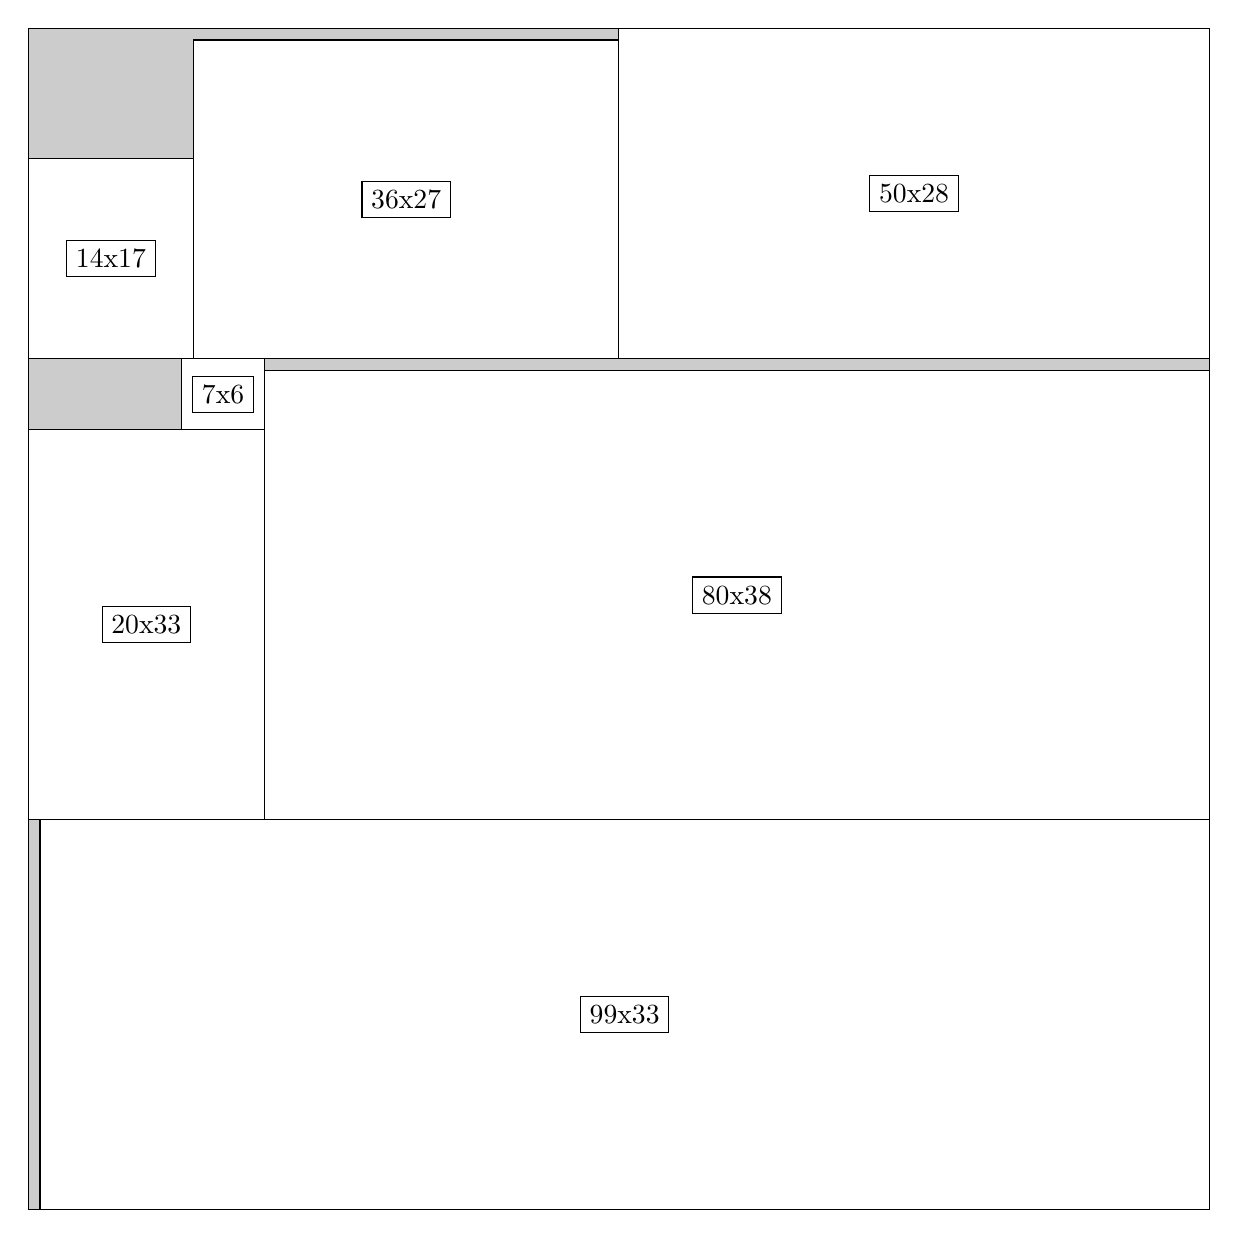
\begin{tikzpicture}[shorten >=1pt,scale=1.0,every node/.style={scale=1.0},->]
\tikzstyle{vertex}=[circle,fill=black!25,minimum size=14pt,inner sep=0pt]
\filldraw[fill=gray!40!white, draw=black] (0,0) rectangle (15.0,15.0);
\foreach \name/\x/\y/\w/\h in {99x33/0.15/0.0/14.85/4.95,80x38/3.0/4.95/12.0/5.7,20x33/0.0/4.95/3.0/4.95,7x6/1.95/9.9/1.05/0.8999999999999999,50x28/7.5/10.799999999999999/7.5/4.2,36x27/2.1/10.799999999999999/5.3999999999999995/4.05,14x17/0.0/10.799999999999999/2.1/2.55}
\filldraw[fill=white!40!white, draw=black] (\x,\y) rectangle node[draw] (\name) {\name} ++(\w,\h);
\end{tikzpicture}


w =99 , h =33 , x =1 , y =0 , v =3267
\par
w =80 , h =38 , x =20 , y =33 , v =3040
\par
w =20 , h =33 , x =0 , y =33 , v =660
\par
w =7 , h =6 , x =13 , y =66 , v =42
\par
w =50 , h =28 , x =50 , y =72 , v =1400
\par
w =36 , h =27 , x =14 , y =72 , v =972
\par
w =14 , h =17 , x =0 , y =72 , v =238
\par
\newpage


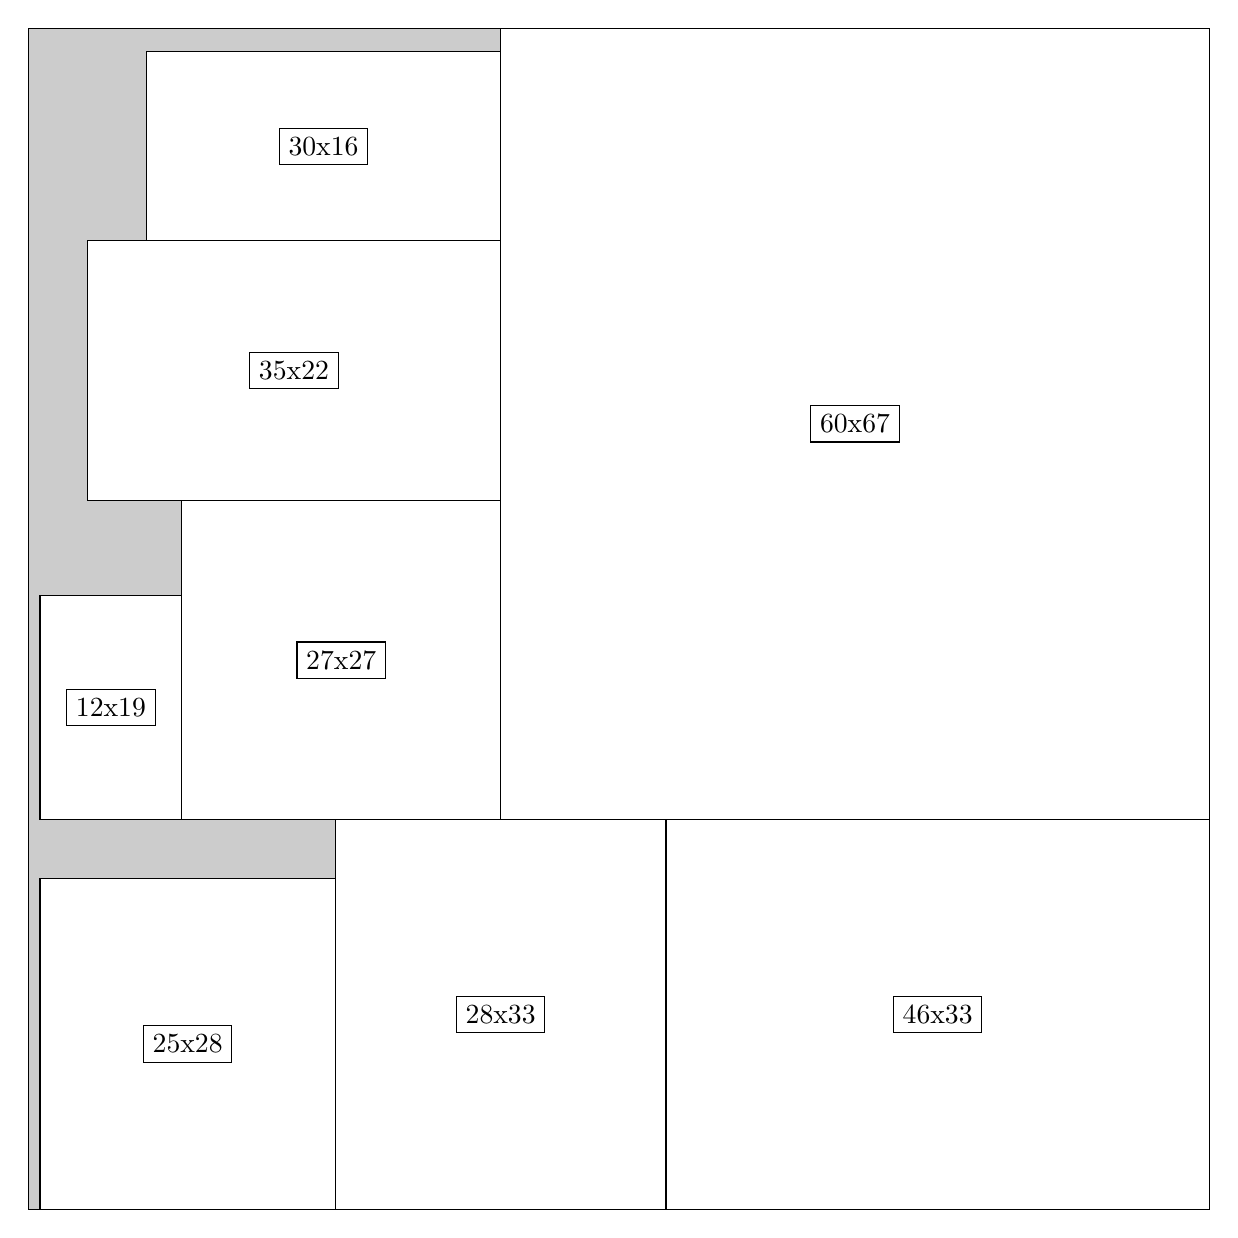
\begin{tikzpicture}[shorten >=1pt,scale=1.0,every node/.style={scale=1.0},->]
\tikzstyle{vertex}=[circle,fill=black!25,minimum size=14pt,inner sep=0pt]
\filldraw[fill=gray!40!white, draw=black] (0,0) rectangle (15.0,15.0);
\foreach \name/\x/\y/\w/\h in {46x33/8.1/0.0/6.8999999999999995/4.95,28x33/3.9/0.0/4.2/4.95,25x28/0.15/0.0/3.75/4.2,60x67/6.0/4.95/9.0/10.049999999999999,27x27/1.95/4.95/4.05/4.05,12x19/0.15/4.95/1.7999999999999998/2.85,35x22/0.75/9.0/5.25/3.3,30x16/1.5/12.299999999999999/4.5/2.4}
\filldraw[fill=white!40!white, draw=black] (\x,\y) rectangle node[draw] (\name) {\name} ++(\w,\h);
\end{tikzpicture}


w =46 , h =33 , x =54 , y =0 , v =1518
\par
w =28 , h =33 , x =26 , y =0 , v =924
\par
w =25 , h =28 , x =1 , y =0 , v =700
\par
w =60 , h =67 , x =40 , y =33 , v =4020
\par
w =27 , h =27 , x =13 , y =33 , v =729
\par
w =12 , h =19 , x =1 , y =33 , v =228
\par
w =35 , h =22 , x =5 , y =60 , v =770
\par
w =30 , h =16 , x =10 , y =82 , v =480
\par
\newpage


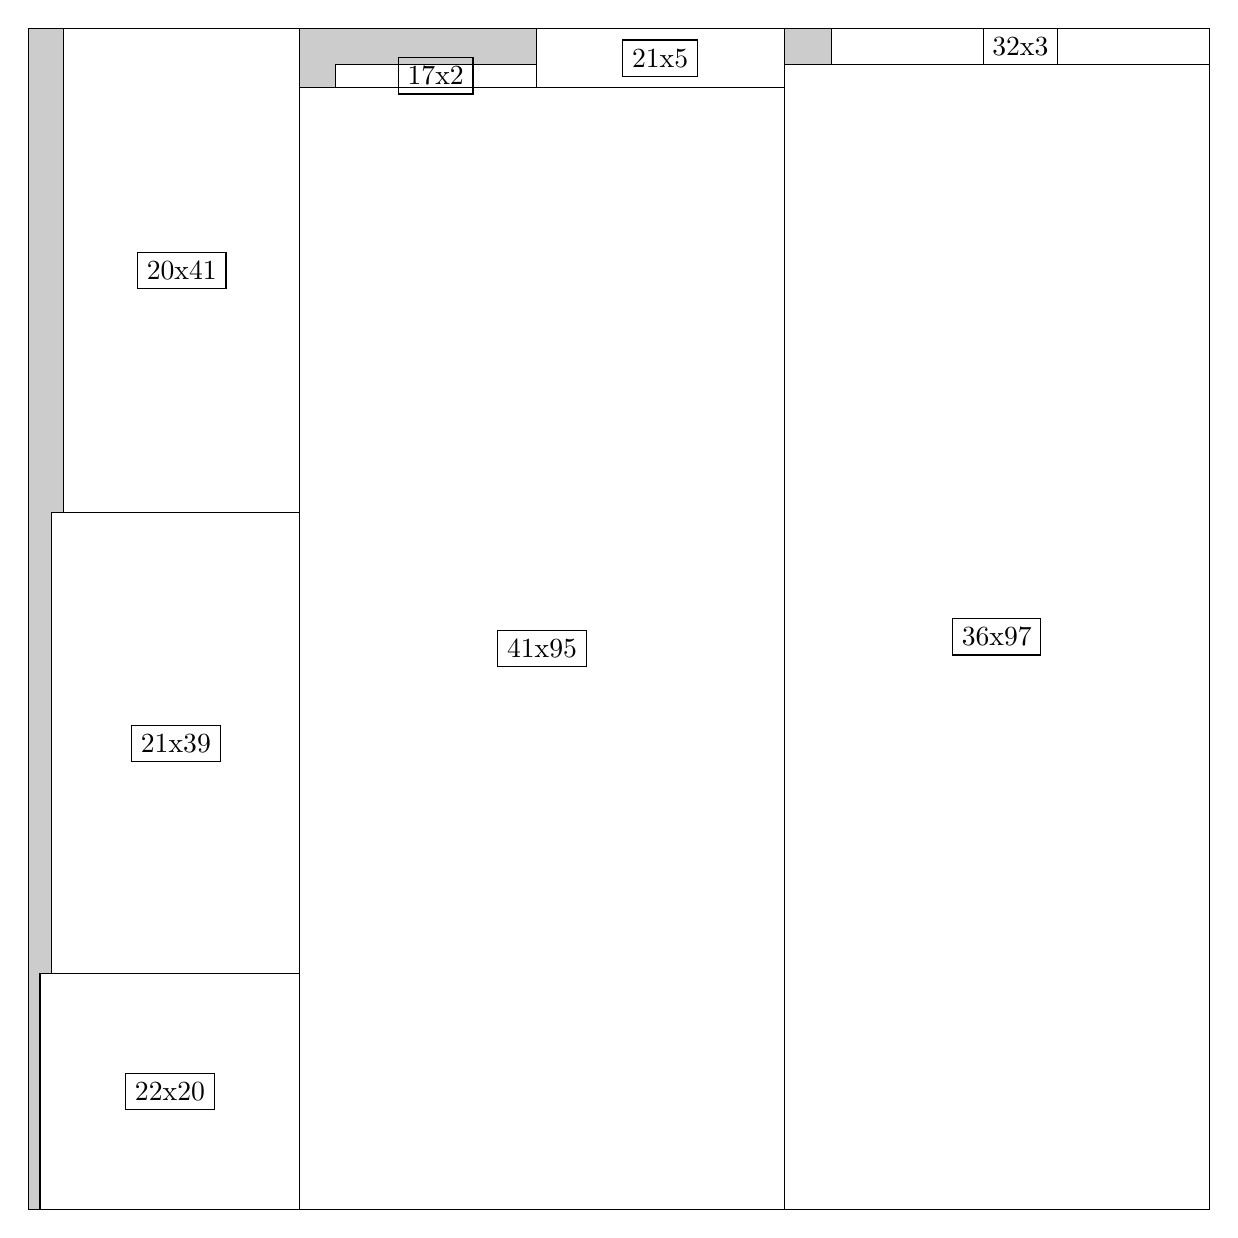
\begin{tikzpicture}[shorten >=1pt,scale=1.0,every node/.style={scale=1.0},->]
\tikzstyle{vertex}=[circle,fill=black!25,minimum size=14pt,inner sep=0pt]
\filldraw[fill=gray!40!white, draw=black] (0,0) rectangle (15.0,15.0);
\foreach \name/\x/\y/\w/\h in {36x97/9.6/0.0/5.3999999999999995/14.549999999999999,32x3/10.2/14.549999999999999/4.8/0.44999999999999996,41x95/3.4499999999999997/0.0/6.1499999999999995/14.25,21x5/6.45/14.25/3.15/0.75,17x2/3.9/14.25/2.55/0.3,22x20/0.15/0.0/3.3/3.0,21x39/0.3/3.0/3.15/5.85,20x41/0.44999999999999996/8.85/3.0/6.1499999999999995}
\filldraw[fill=white!40!white, draw=black] (\x,\y) rectangle node[draw] (\name) {\name} ++(\w,\h);
\end{tikzpicture}


w =36 , h =97 , x =64 , y =0 , v =3492
\par
w =32 , h =3 , x =68 , y =97 , v =96
\par
w =41 , h =95 , x =23 , y =0 , v =3895
\par
w =21 , h =5 , x =43 , y =95 , v =105
\par
w =17 , h =2 , x =26 , y =95 , v =34
\par
w =22 , h =20 , x =1 , y =0 , v =440
\par
w =21 , h =39 , x =2 , y =20 , v =819
\par
w =20 , h =41 , x =3 , y =59 , v =820
\par
\newpage


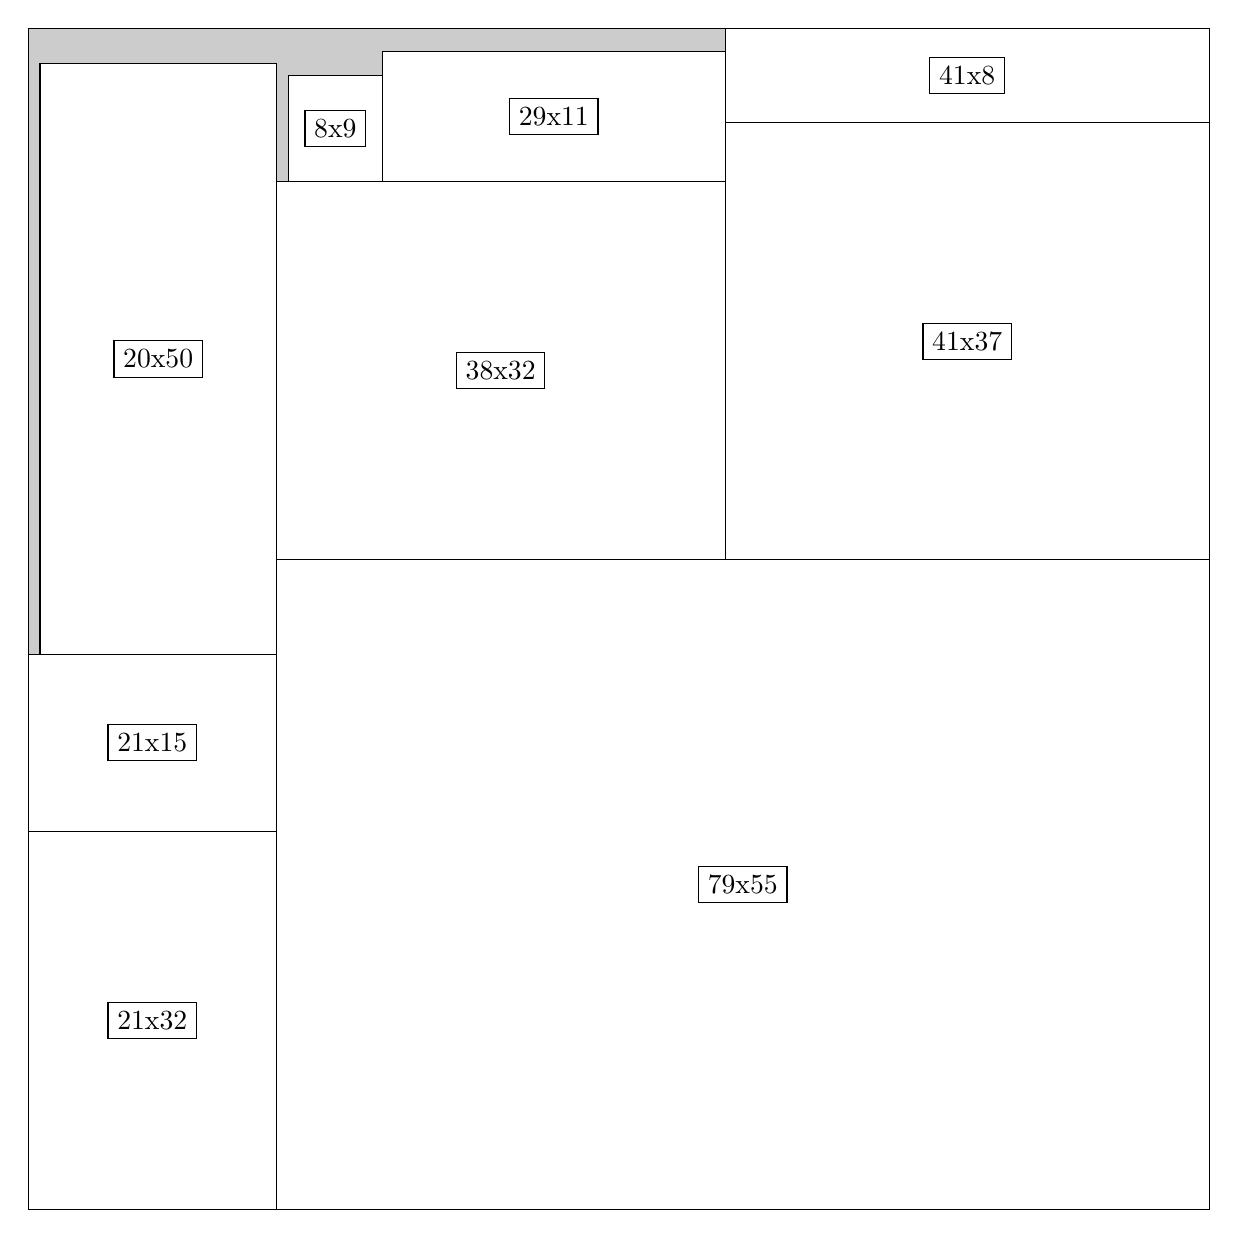
\begin{tikzpicture}[shorten >=1pt,scale=1.0,every node/.style={scale=1.0},->]
\tikzstyle{vertex}=[circle,fill=black!25,minimum size=14pt,inner sep=0pt]
\filldraw[fill=gray!40!white, draw=black] (0,0) rectangle (15.0,15.0);
\foreach \name/\x/\y/\w/\h in {79x55/3.15/0.0/11.85/8.25,41x37/8.85/8.25/6.1499999999999995/5.55,41x8/8.85/13.799999999999999/6.1499999999999995/1.2,38x32/3.15/8.25/5.7/4.8,29x11/4.5/13.049999999999999/4.35/1.65,8x9/3.3/13.049999999999999/1.2/1.3499999999999999,21x32/0.0/0.0/3.15/4.8,21x15/0.0/4.8/3.15/2.25,20x50/0.15/7.05/3.0/7.5}
\filldraw[fill=white!40!white, draw=black] (\x,\y) rectangle node[draw] (\name) {\name} ++(\w,\h);
\end{tikzpicture}


w =79 , h =55 , x =21 , y =0 , v =4345
\par
w =41 , h =37 , x =59 , y =55 , v =1517
\par
w =41 , h =8 , x =59 , y =92 , v =328
\par
w =38 , h =32 , x =21 , y =55 , v =1216
\par
w =29 , h =11 , x =30 , y =87 , v =319
\par
w =8 , h =9 , x =22 , y =87 , v =72
\par
w =21 , h =32 , x =0 , y =0 , v =672
\par
w =21 , h =15 , x =0 , y =32 , v =315
\par
w =20 , h =50 , x =1 , y =47 , v =1000
\par
\newpage


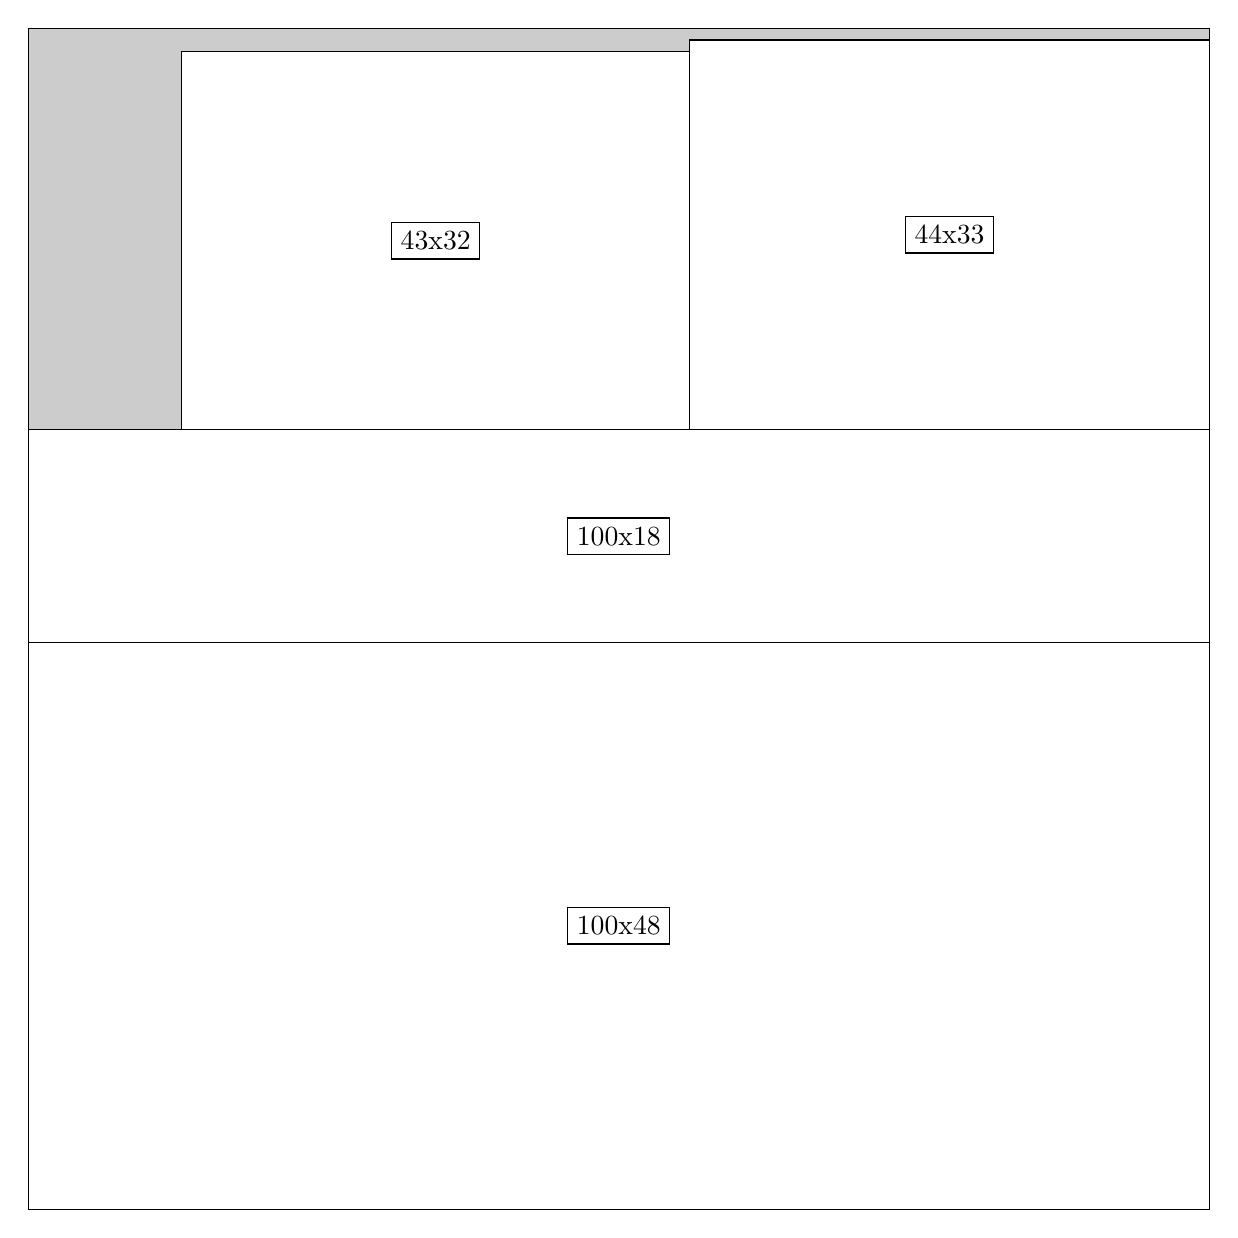
\begin{tikzpicture}[shorten >=1pt,scale=1.0,every node/.style={scale=1.0},->]
\tikzstyle{vertex}=[circle,fill=black!25,minimum size=14pt,inner sep=0pt]
\filldraw[fill=gray!40!white, draw=black] (0,0) rectangle (15.0,15.0);
\foreach \name/\x/\y/\w/\h in {100x48/0.0/0.0/15.0/7.199999999999999,100x18/0.0/7.199999999999999/15.0/2.6999999999999997,44x33/8.4/9.9/6.6/4.95,43x32/1.95/9.9/6.45/4.8}
\filldraw[fill=white!40!white, draw=black] (\x,\y) rectangle node[draw] (\name) {\name} ++(\w,\h);
\end{tikzpicture}


w =100 , h =48 , x =0 , y =0 , v =4800
\par
w =100 , h =18 , x =0 , y =48 , v =1800
\par
w =44 , h =33 , x =56 , y =66 , v =1452
\par
w =43 , h =32 , x =13 , y =66 , v =1376
\par
\newpage


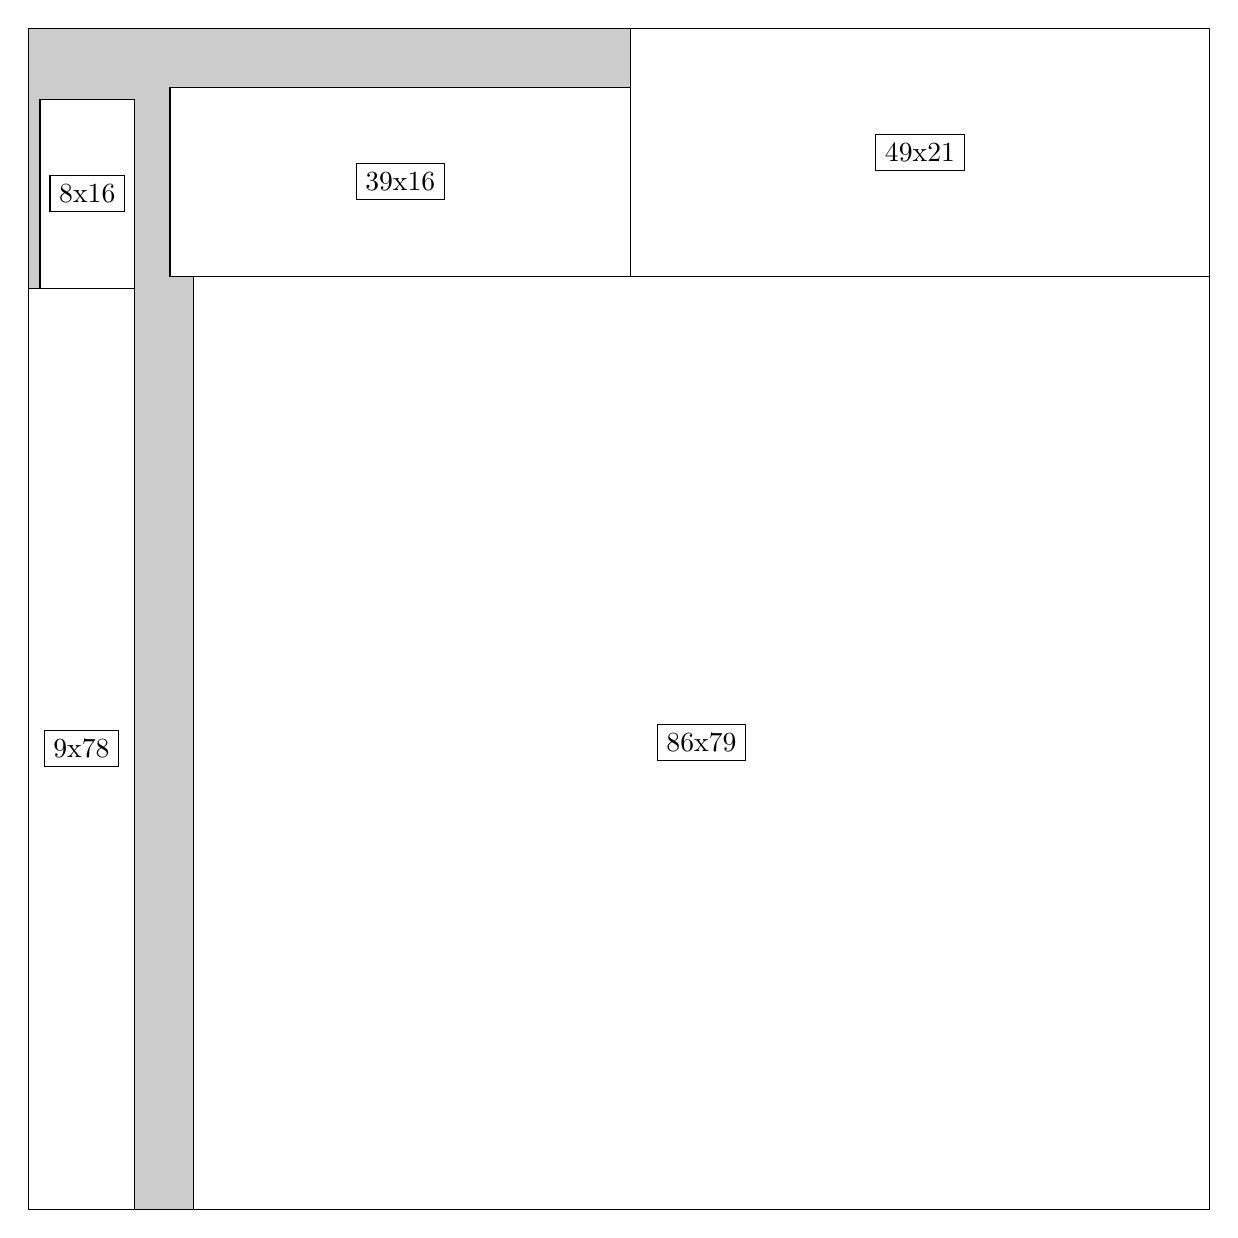
\begin{tikzpicture}[shorten >=1pt,scale=1.0,every node/.style={scale=1.0},->]
\tikzstyle{vertex}=[circle,fill=black!25,minimum size=14pt,inner sep=0pt]
\filldraw[fill=gray!40!white, draw=black] (0,0) rectangle (15.0,15.0);
\foreach \name/\x/\y/\w/\h in {86x79/2.1/0.0/12.9/11.85,49x21/7.6499999999999995/11.85/7.35/3.15,39x16/1.7999999999999998/11.85/5.85/2.4,9x78/0.0/0.0/1.3499999999999999/11.7,8x16/0.15/11.7/1.2/2.4}
\filldraw[fill=white!40!white, draw=black] (\x,\y) rectangle node[draw] (\name) {\name} ++(\w,\h);
\end{tikzpicture}


w =86 , h =79 , x =14 , y =0 , v =6794
\par
w =49 , h =21 , x =51 , y =79 , v =1029
\par
w =39 , h =16 , x =12 , y =79 , v =624
\par
w =9 , h =78 , x =0 , y =0 , v =702
\par
w =8 , h =16 , x =1 , y =78 , v =128
\par
\newpage



\begin{tikzpicture}[shorten >=1pt,scale=1.0,every node/.style={scale=1.0},->]
\tikzstyle{vertex}=[circle,fill=black!25,minimum size=14pt,inner sep=0pt]
\filldraw[fill=gray!40!white, draw=black] (0,0) rectangle (15.0,15.0);
\foreach \name/\x/\y/\w/\h in {94x98/0.8999999999999999/0.0/14.1/14.7}
\filldraw[fill=white!40!white, draw=black] (\x,\y) rectangle node[draw] (\name) {\name} ++(\w,\h);
\end{tikzpicture}


w =94 , h =98 , x =6 , y =0 , v =9212
\par
\newpage


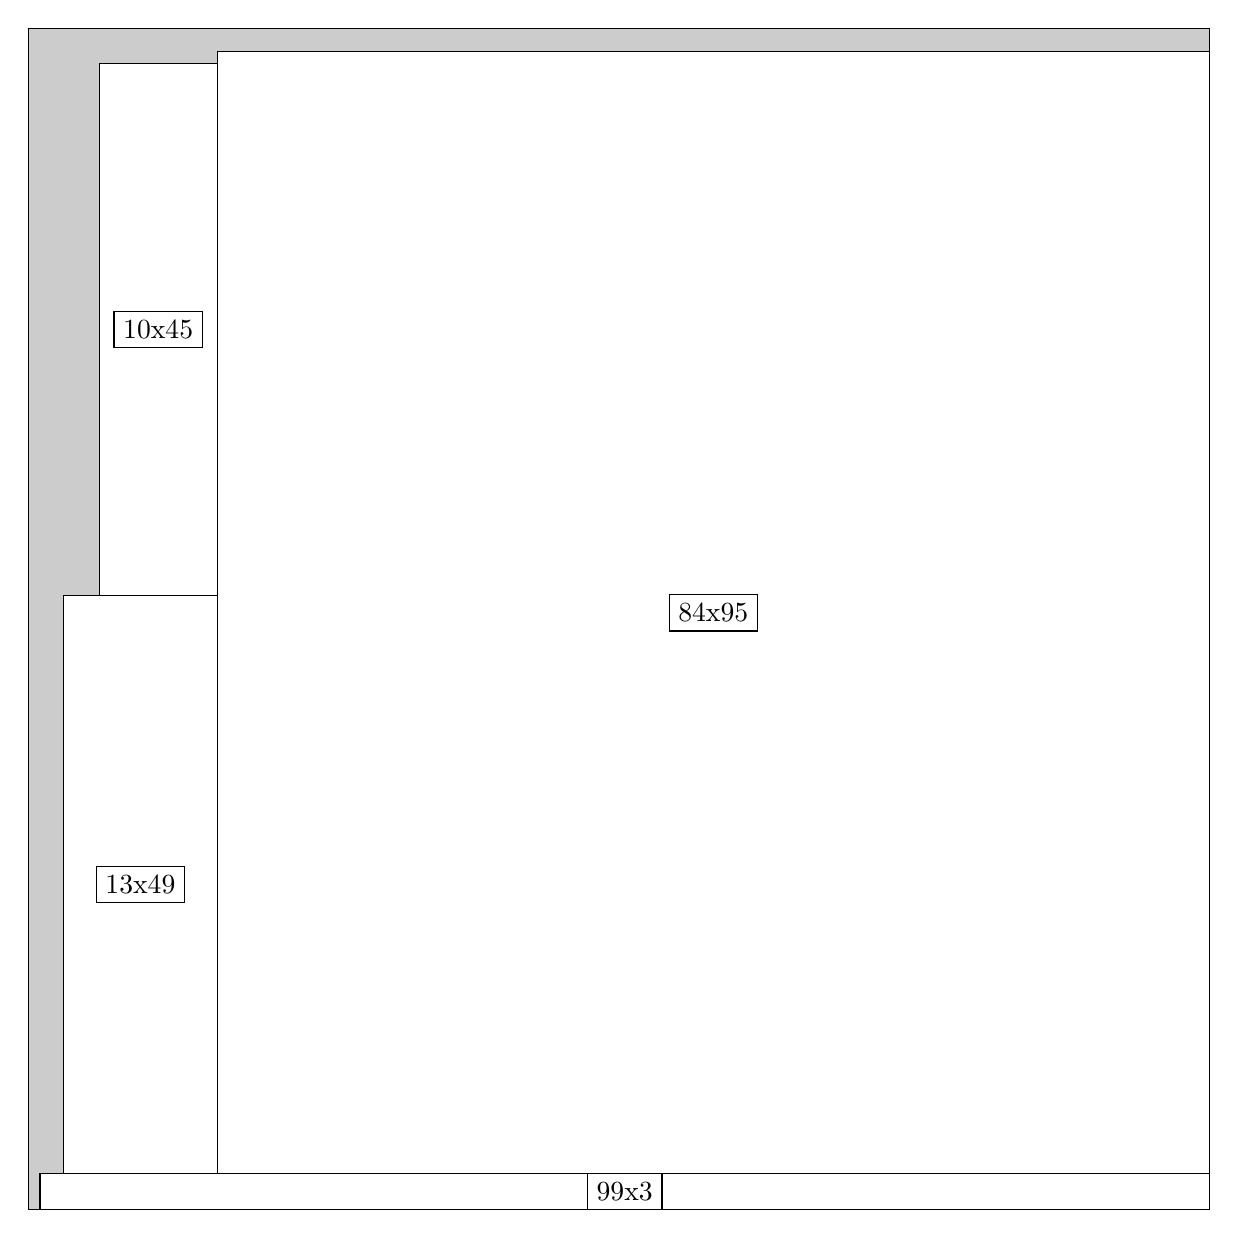
\begin{tikzpicture}[shorten >=1pt,scale=1.0,every node/.style={scale=1.0},->]
\tikzstyle{vertex}=[circle,fill=black!25,minimum size=14pt,inner sep=0pt]
\filldraw[fill=gray!40!white, draw=black] (0,0) rectangle (15.0,15.0);
\foreach \name/\x/\y/\w/\h in {99x3/0.15/0.0/14.85/0.44999999999999996,84x95/2.4/0.44999999999999996/12.6/14.25,13x49/0.44999999999999996/0.44999999999999996/1.95/7.35,10x45/0.8999999999999999/7.8/1.5/6.75}
\filldraw[fill=white!40!white, draw=black] (\x,\y) rectangle node[draw] (\name) {\name} ++(\w,\h);
\end{tikzpicture}


w =99 , h =3 , x =1 , y =0 , v =297
\par
w =84 , h =95 , x =16 , y =3 , v =7980
\par
w =13 , h =49 , x =3 , y =3 , v =637
\par
w =10 , h =45 , x =6 , y =52 , v =450
\par
\newpage


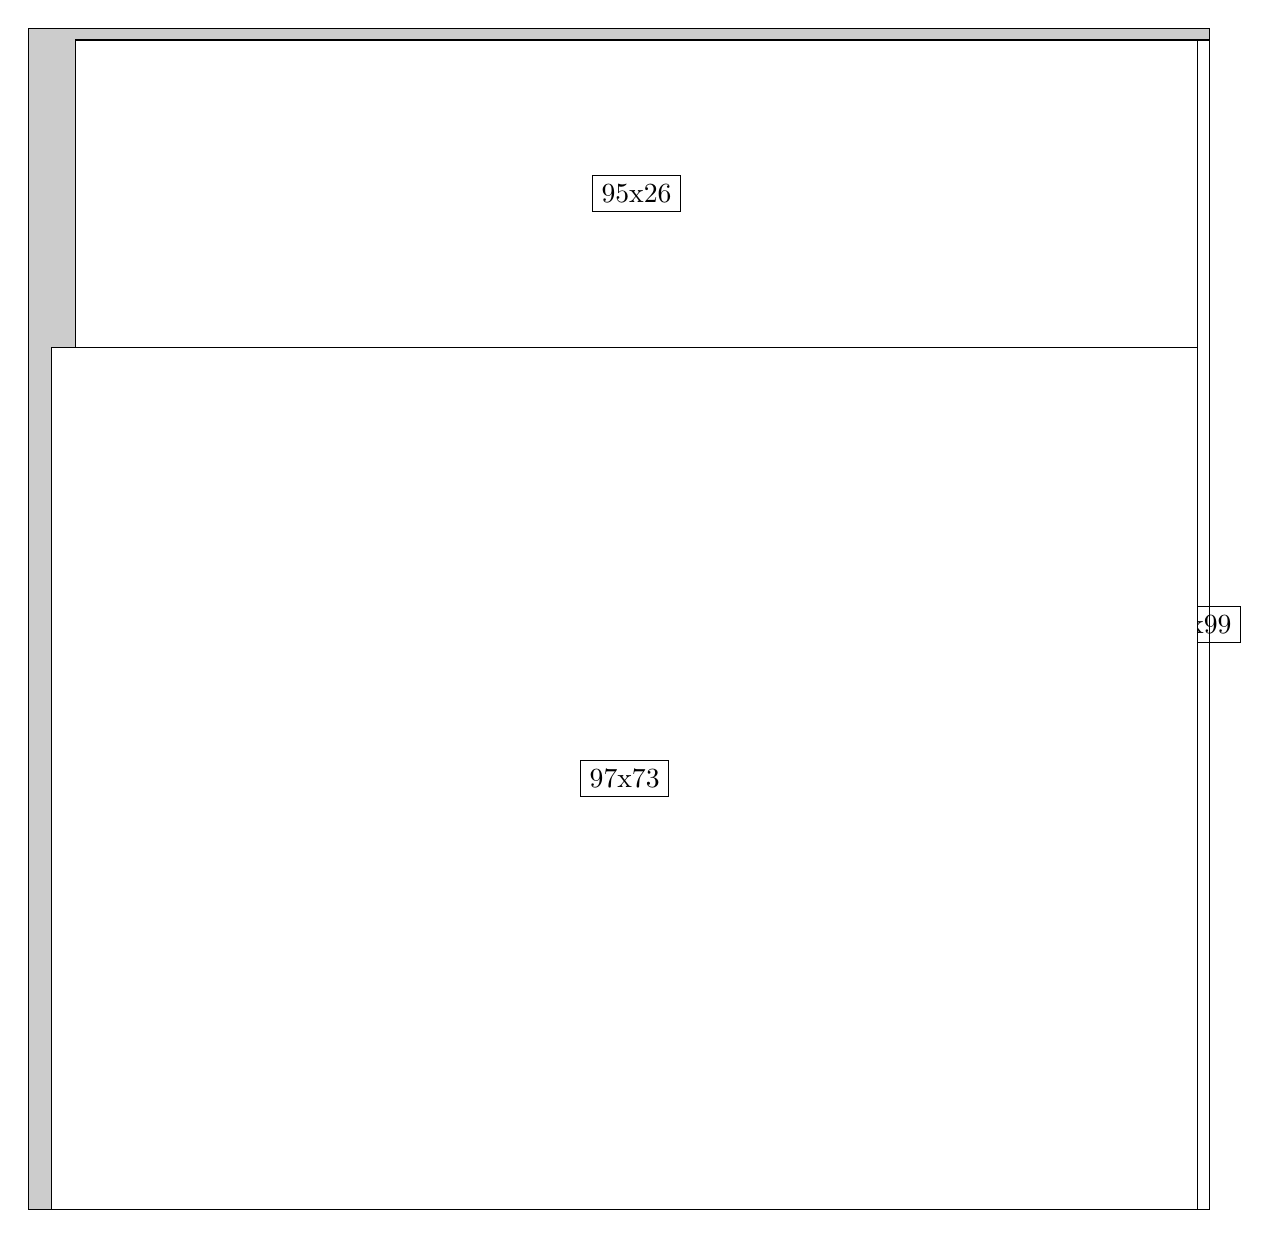
\begin{tikzpicture}[shorten >=1pt,scale=1.0,every node/.style={scale=1.0},->]
\tikzstyle{vertex}=[circle,fill=black!25,minimum size=14pt,inner sep=0pt]
\filldraw[fill=gray!40!white, draw=black] (0,0) rectangle (15.0,15.0);
\foreach \name/\x/\y/\w/\h in {1x99/14.85/0.0/0.15/14.85,97x73/0.3/0.0/14.549999999999999/10.95,95x26/0.6/10.95/14.25/3.9}
\filldraw[fill=white!40!white, draw=black] (\x,\y) rectangle node[draw] (\name) {\name} ++(\w,\h);
\end{tikzpicture}


w =1 , h =99 , x =99 , y =0 , v =99
\par
w =97 , h =73 , x =2 , y =0 , v =7081
\par
w =95 , h =26 , x =4 , y =73 , v =2470
\par
\newpage


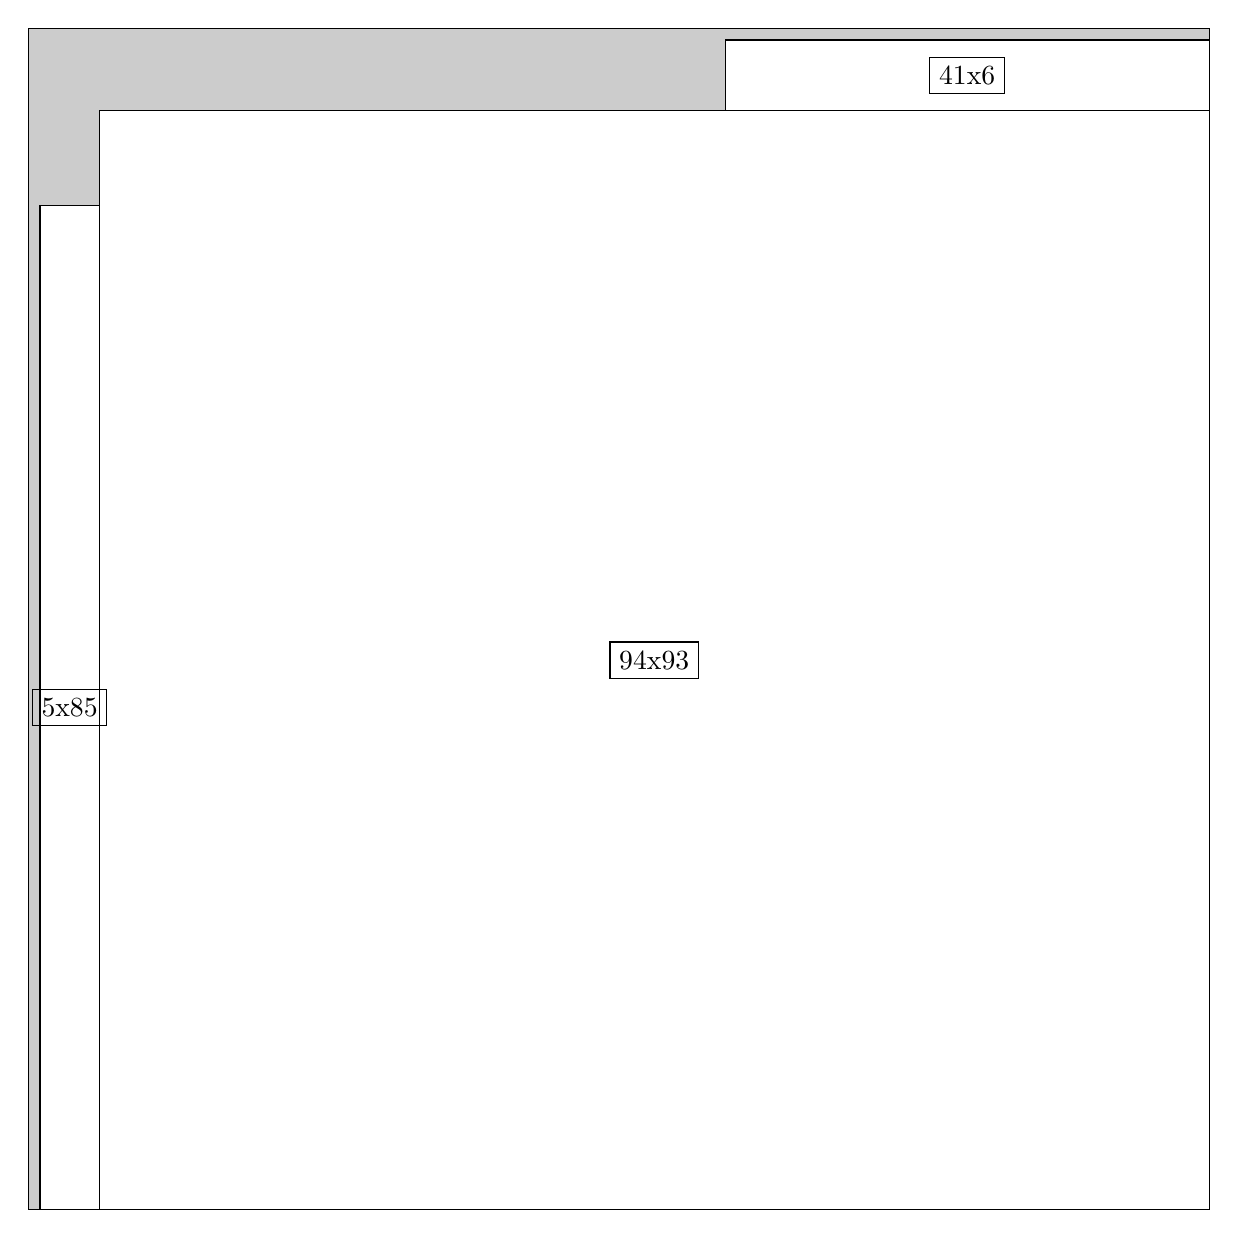
\begin{tikzpicture}[shorten >=1pt,scale=1.0,every node/.style={scale=1.0},->]
\tikzstyle{vertex}=[circle,fill=black!25,minimum size=14pt,inner sep=0pt]
\filldraw[fill=gray!40!white, draw=black] (0,0) rectangle (15.0,15.0);
\foreach \name/\x/\y/\w/\h in {94x93/0.8999999999999999/0.0/14.1/13.95,5x85/0.15/0.0/0.75/12.75,41x6/8.85/13.95/6.1499999999999995/0.8999999999999999}
\filldraw[fill=white!40!white, draw=black] (\x,\y) rectangle node[draw] (\name) {\name} ++(\w,\h);
\end{tikzpicture}


w =94 , h =93 , x =6 , y =0 , v =8742
\par
w =5 , h =85 , x =1 , y =0 , v =425
\par
w =41 , h =6 , x =59 , y =93 , v =246
\par
\newpage


\end{document}